\documentclass[]{book}
\usepackage{lmodern}
\usepackage{amssymb,amsmath}
\usepackage{ifxetex,ifluatex}
\usepackage{fixltx2e} % provides \textsubscript
\ifnum 0\ifxetex 1\fi\ifluatex 1\fi=0 % if pdftex
  \usepackage[T1]{fontenc}
  \usepackage[utf8]{inputenc}
\else % if luatex or xelatex
  \ifxetex
    \usepackage{mathspec}
  \else
    \usepackage{fontspec}
  \fi
  \defaultfontfeatures{Ligatures=TeX,Scale=MatchLowercase}
\fi
% use upquote if available, for straight quotes in verbatim environments
\IfFileExists{upquote.sty}{\usepackage{upquote}}{}
% use microtype if available
\IfFileExists{microtype.sty}{%
\usepackage{microtype}
\UseMicrotypeSet[protrusion]{basicmath} % disable protrusion for tt fonts
}{}
\usepackage{hyperref}
\hypersetup{unicode=true,
            pdftitle={Global Fund eTracker: Technical Guide},
            pdfauthor={Isaiah Nyabuto, Cristina Lussiana},
            pdfborder={0 0 0},
            breaklinks=true}
\urlstyle{same}  % don't use monospace font for urls
\usepackage{natbib}
\bibliographystyle{apalike}
\usepackage{longtable,booktabs}
\usepackage{graphicx,grffile}
\makeatletter
\def\maxwidth{\ifdim\Gin@nat@width>\linewidth\linewidth\else\Gin@nat@width\fi}
\def\maxheight{\ifdim\Gin@nat@height>\textheight\textheight\else\Gin@nat@height\fi}
\makeatother
% Scale images if necessary, so that they will not overflow the page
% margins by default, and it is still possible to overwrite the defaults
% using explicit options in \includegraphics[width, height, ...]{}
\setkeys{Gin}{width=\maxwidth,height=\maxheight,keepaspectratio}
\IfFileExists{parskip.sty}{%
\usepackage{parskip}
}{% else
\setlength{\parindent}{0pt}
\setlength{\parskip}{6pt plus 2pt minus 1pt}
}
\setlength{\emergencystretch}{3em}  % prevent overfull lines
\providecommand{\tightlist}{%
  \setlength{\itemsep}{0pt}\setlength{\parskip}{0pt}}
\setcounter{secnumdepth}{5}
% Redefines (sub)paragraphs to behave more like sections
\ifx\paragraph\undefined\else
\let\oldparagraph\paragraph
\renewcommand{\paragraph}[1]{\oldparagraph{#1}\mbox{}}
\fi
\ifx\subparagraph\undefined\else
\let\oldsubparagraph\subparagraph
\renewcommand{\subparagraph}[1]{\oldsubparagraph{#1}\mbox{}}
\fi

%%% Use protect on footnotes to avoid problems with footnotes in titles
\let\rmarkdownfootnote\footnote%
\def\footnote{\protect\rmarkdownfootnote}

%%% Change title format to be more compact
\usepackage{titling}

% Create subtitle command for use in maketitle
\providecommand{\subtitle}[1]{
  \posttitle{
    \begin{center}\large#1\end{center}
    }
}

\setlength{\droptitle}{-2em}

  \title{Global Fund eTracker: Technical Guide}
    \pretitle{\vspace{\droptitle}\centering\huge}
  \posttitle{\par}
    \author{Isaiah Nyabuto, Cristina Lussiana}
    \preauthor{\centering\large\emph}
  \postauthor{\par}
      \predate{\centering\large\emph}
  \postdate{\par}
    \date{2019-10-09}

\usepackage{booktabs}

\begin{document}
\maketitle

{
\setcounter{tocdepth}{1}
\tableofcontents
}
\hypertarget{preface}{%
\chapter*{Preface}\label{preface}}
\addcontentsline{toc}{chapter}{Preface}


\includegraphics{./images/gf_logo copy.jpg}

\hypertarget{introduction}{%
\chapter{Introduction}\label{introduction}}

\hypertarget{purpose}{%
\section{Purpose}\label{purpose}}

The goal of this job aid is to describe the overall system implementation of the Global Fund eTracker and provide guidance on further development and customization of the tool. Global Fund eTracker is a data reporting tool that provides more visibility on the GF metrics and helps to align the project's target with the current progress.

\hypertarget{document-convention}{%
\section{Document Convention}\label{document-convention}}

The guide uses the following conventions;

\begin{longtable}[]{@{}lc@{}}
\toprule
\textbf{Abbreviation} & \textbf{Description}\tabularnewline
\midrule
\endhead
DHIS2 & District Health Information System\tabularnewline
GF & Global Fund\tabularnewline
GBS & Global Business Systems\tabularnewline
GFMU & Global Fund Management Unit\tabularnewline
\bottomrule
\end{longtable}

\begin{center}\rule{0.5\linewidth}{\linethickness}\end{center}

\hypertarget{intended-audience-and-reading-suggestions}{%
\section{Intended Audience and Reading Suggestions}\label{intended-audience-and-reading-suggestions}}

This job aid is intended for DHIS2 implementers and experts, and this includes Architects and support specialists.

\hypertarget{project-scope}{%
\section{Project Scope}\label{project-scope}}

Global Fund eTracker is a data reporting tool designed through a collaboration by GFMU and GBS teams to help provide more visibility on the GF metrics and in the alignment of the project target with the current progress. It supports the GFMU teams in the identification of gaps, monitoring of progress, and to compare the bi-yearly reports prepared by GF countries. The project is active in five countries, and this includes Liberia, Mali, Madagascar, South Sudan, and Haiti.

\hypertarget{references}{%
\section{References}\label{references}}

\begin{itemize}
\tightlist
\item
  \href{https://psiorg.sharepoint.com/:w:/r/sites/us_globalfunde-tracker/_layouts/15/Doc.aspx?sourcedoc=\%7B9D6D6FC8-7EC5-4D8C-8031-7EF2CF247D7E\%7D\&file=GF\%20Tracker\%20One-Pager.docx\&action=default\&mobileredirect=true}{Global Fund One Pager}
\item
  PSI DHIS2 Standards
\item
  Global Fund Indicator Matrix
\end{itemize}

\hypertarget{intro}{%
\chapter{Overall Description}\label{intro}}

\hypertarget{global-fund-etracker-perspective}{%
\section{Global Fund eTracker Perspective}\label{global-fund-etracker-perspective}}

Global Fund eTracker reports information from the following programs;

\begin{itemize}
\tightlist
\item
  HIV/AIDs: This includes the following modules; Comprehensive prevention program for different targets groups and PMTCT.
\item
  Tuberculosis: Includes TB care and prevention, TB / HIV, MDR-TB and Treatment Care Support programs.
\item
  Malaria: Includes Vector Control, HSS -- Procurement and Supply Chain Management, Case management, Health Community Work Force, Specific Prevention Interventions (SPIs).
\end{itemize}

\begin{quote}
Health Information Systems \& M\&E cut across all the three health areas.
\end{quote}

Data is collected in modules within the Global Fund programs through country-specific reporting tools, and then harmonized in a central database for processing and decision making by GFMU.

\begin{figure}

{\centering 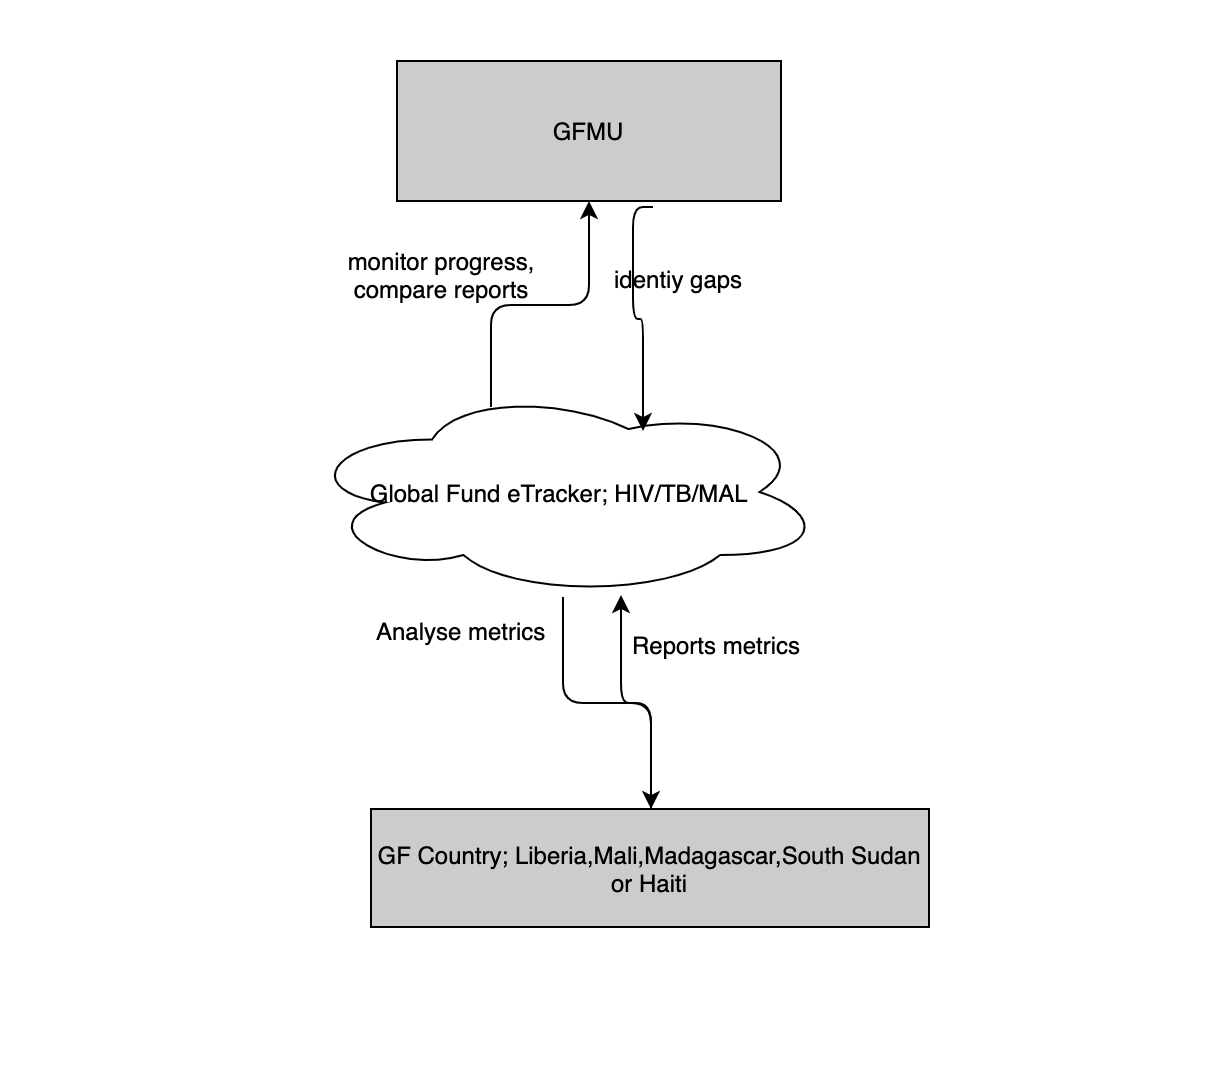
\includegraphics[width=0.8\linewidth]{./images/Screenshot 2019-09-17 at 20.03.42} 

}

\caption{Global Fund eTracker Information Flow}\label{fig:nice-fig}
\end{figure}

\hypertarget{function-specification}{%
\section{Function specification}\label{function-specification}}

Global Fund eTracker features are described below;

\hypertarget{data-specification}{%
\chapter{Data Specification}\label{data-specification}}

\hypertarget{metadata-types}{%
\section{Metadata Types}\label{metadata-types}}

Metadata are helpful to organize the different types of information collected by the Global Fund Management Unit. While other metadata may be included based on a country reporting need, the Global Fund eTracker implements the following metadata types.

\label{tab:nice-tab}A description of Global Fund eTracker Metadata Types

Metadata

Description

Data elements

Description

Data elements forms the basis of the Global Fund eTracker. They define what is recorded in the system.GF eTracker data elements follows PSI DHIS2 standards for names and short names \& the GF Indicator matrix for the form names.

For instance: GF HIV/AIDS - Estimated MSMs is a data element that records the estimated number of MSMs in a region.

Date element groups

Description

Data element groups provides a mechanism for classifying Global Fund related data elements into a common theme.

For instance: GF Malaria groups together all GF Malaria data elements.

Data sets

Description

Data reporting in the Global Fund eTracker is organized through the use of the use of data sets.

A data set is a collection of data elements grouped together for data collection.

For instance: GF HT - HIV/AIDs is used to report data from HIV/AIDs program in Haiti (HT).

Sections

Description

Section are used to split the Global Fund eTracker data sets into small reportable chunks known as modules.

They allow for a bit more flexibility when it comes to using the tabular forms in DHIS2 and are quick and simple to design.

For instance: Comprehensive prevention program for MSMs is a section within the GF HT -- HIV/AIDs data set that groups together indicators to form a module Comprehensive prevention program used in the GF HIV programs.

Category combos

Description

Category combos are used to apply Global Fund disaggregation onto the data elements and indicators.They allow multiple categories to be combined into a related set.

For instance: Number of TB cases with Rifampicin-resistant (RR-TB) and/or MDR-TB notified is disaggregated according to the following categories; Sex (Female, Male) \& Age (\textless{}15; 15+)

Periods

Description

Global Fund eTracker supports DHIS2 standard period types to report and analyze performance over time.

For instance: 201901 to report on January of 2019 or 2019Sn1 to report on the first semester of year 2019.

\hypertarget{standards}{%
\section{Standards}\label{standards}}

Global Fund eTracker leverages PSI DHIS2 standards in metadata configurations and follows the principles for digital technology as the leading standard.

\hypertarget{psi-dhis2-standards}{%
\subsection{PSI DHIS2 Standards}\label{psi-dhis2-standards}}

Similar to the Health Service Report (HSR), data elements are shared and can be re-used across countries. Unlike HSR, Global Fund eTracker implements country-specific data sets and uses the default sections to display forms on the data entry screen.

\hypertarget{global-fund-indicator-framework}{%
\subsection{Global Fund Indicator Framework}\label{global-fund-indicator-framework}}

The Global Fund Indicator Framework guides the reporting and data requirements for the Global Fund eTracker. Countries may have their own specific data or disaggregtions requirements, therefore, the Global Fund eTracker implements country specific reporting tools

\hypertarget{hivtb-blueprint}{%
\subsubsection{HIV/TB Blueprint}\label{hivtb-blueprint}}

\begin{figure}

{\centering 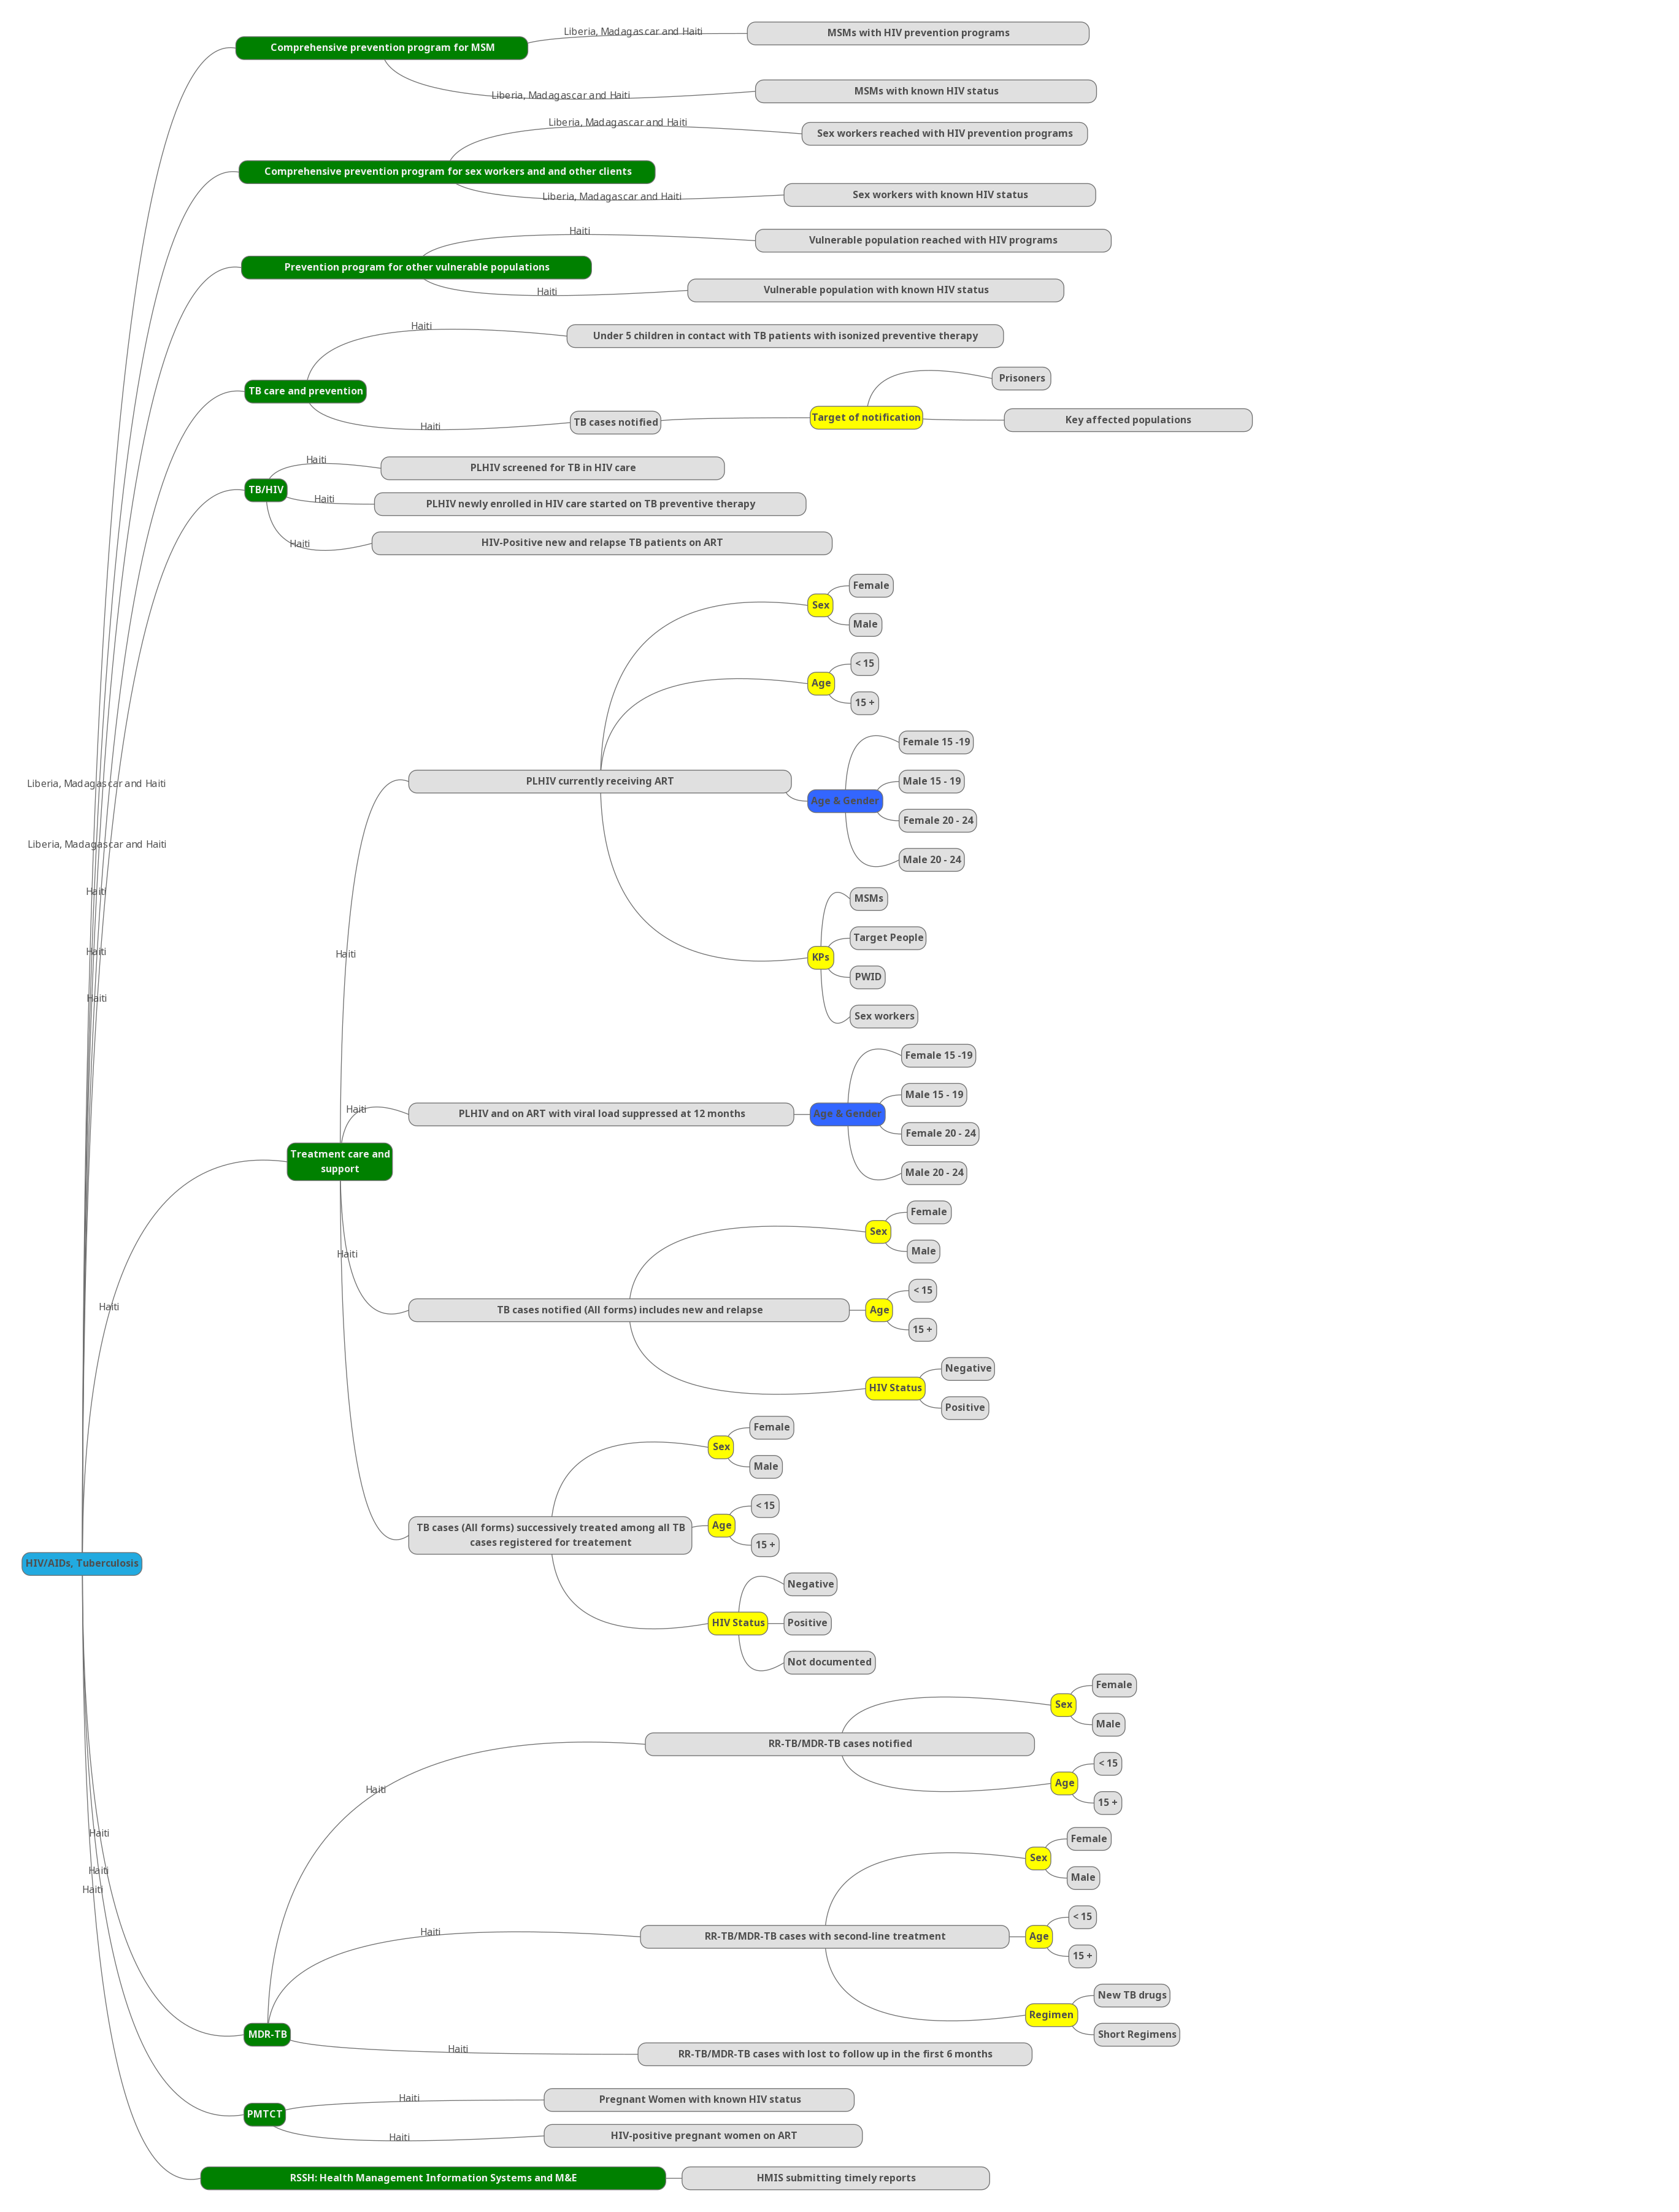
\includegraphics[width=0.8\linewidth]{./images/gfmublueprint} 

}

\caption{Global Fund eTracker blueprint}\label{fig:nice-fig2}
\end{figure}

\hypertarget{malaria-blueprint}{%
\subsubsection{Malaria Blueprint}\label{malaria-blueprint}}

\begin{figure}

{\centering 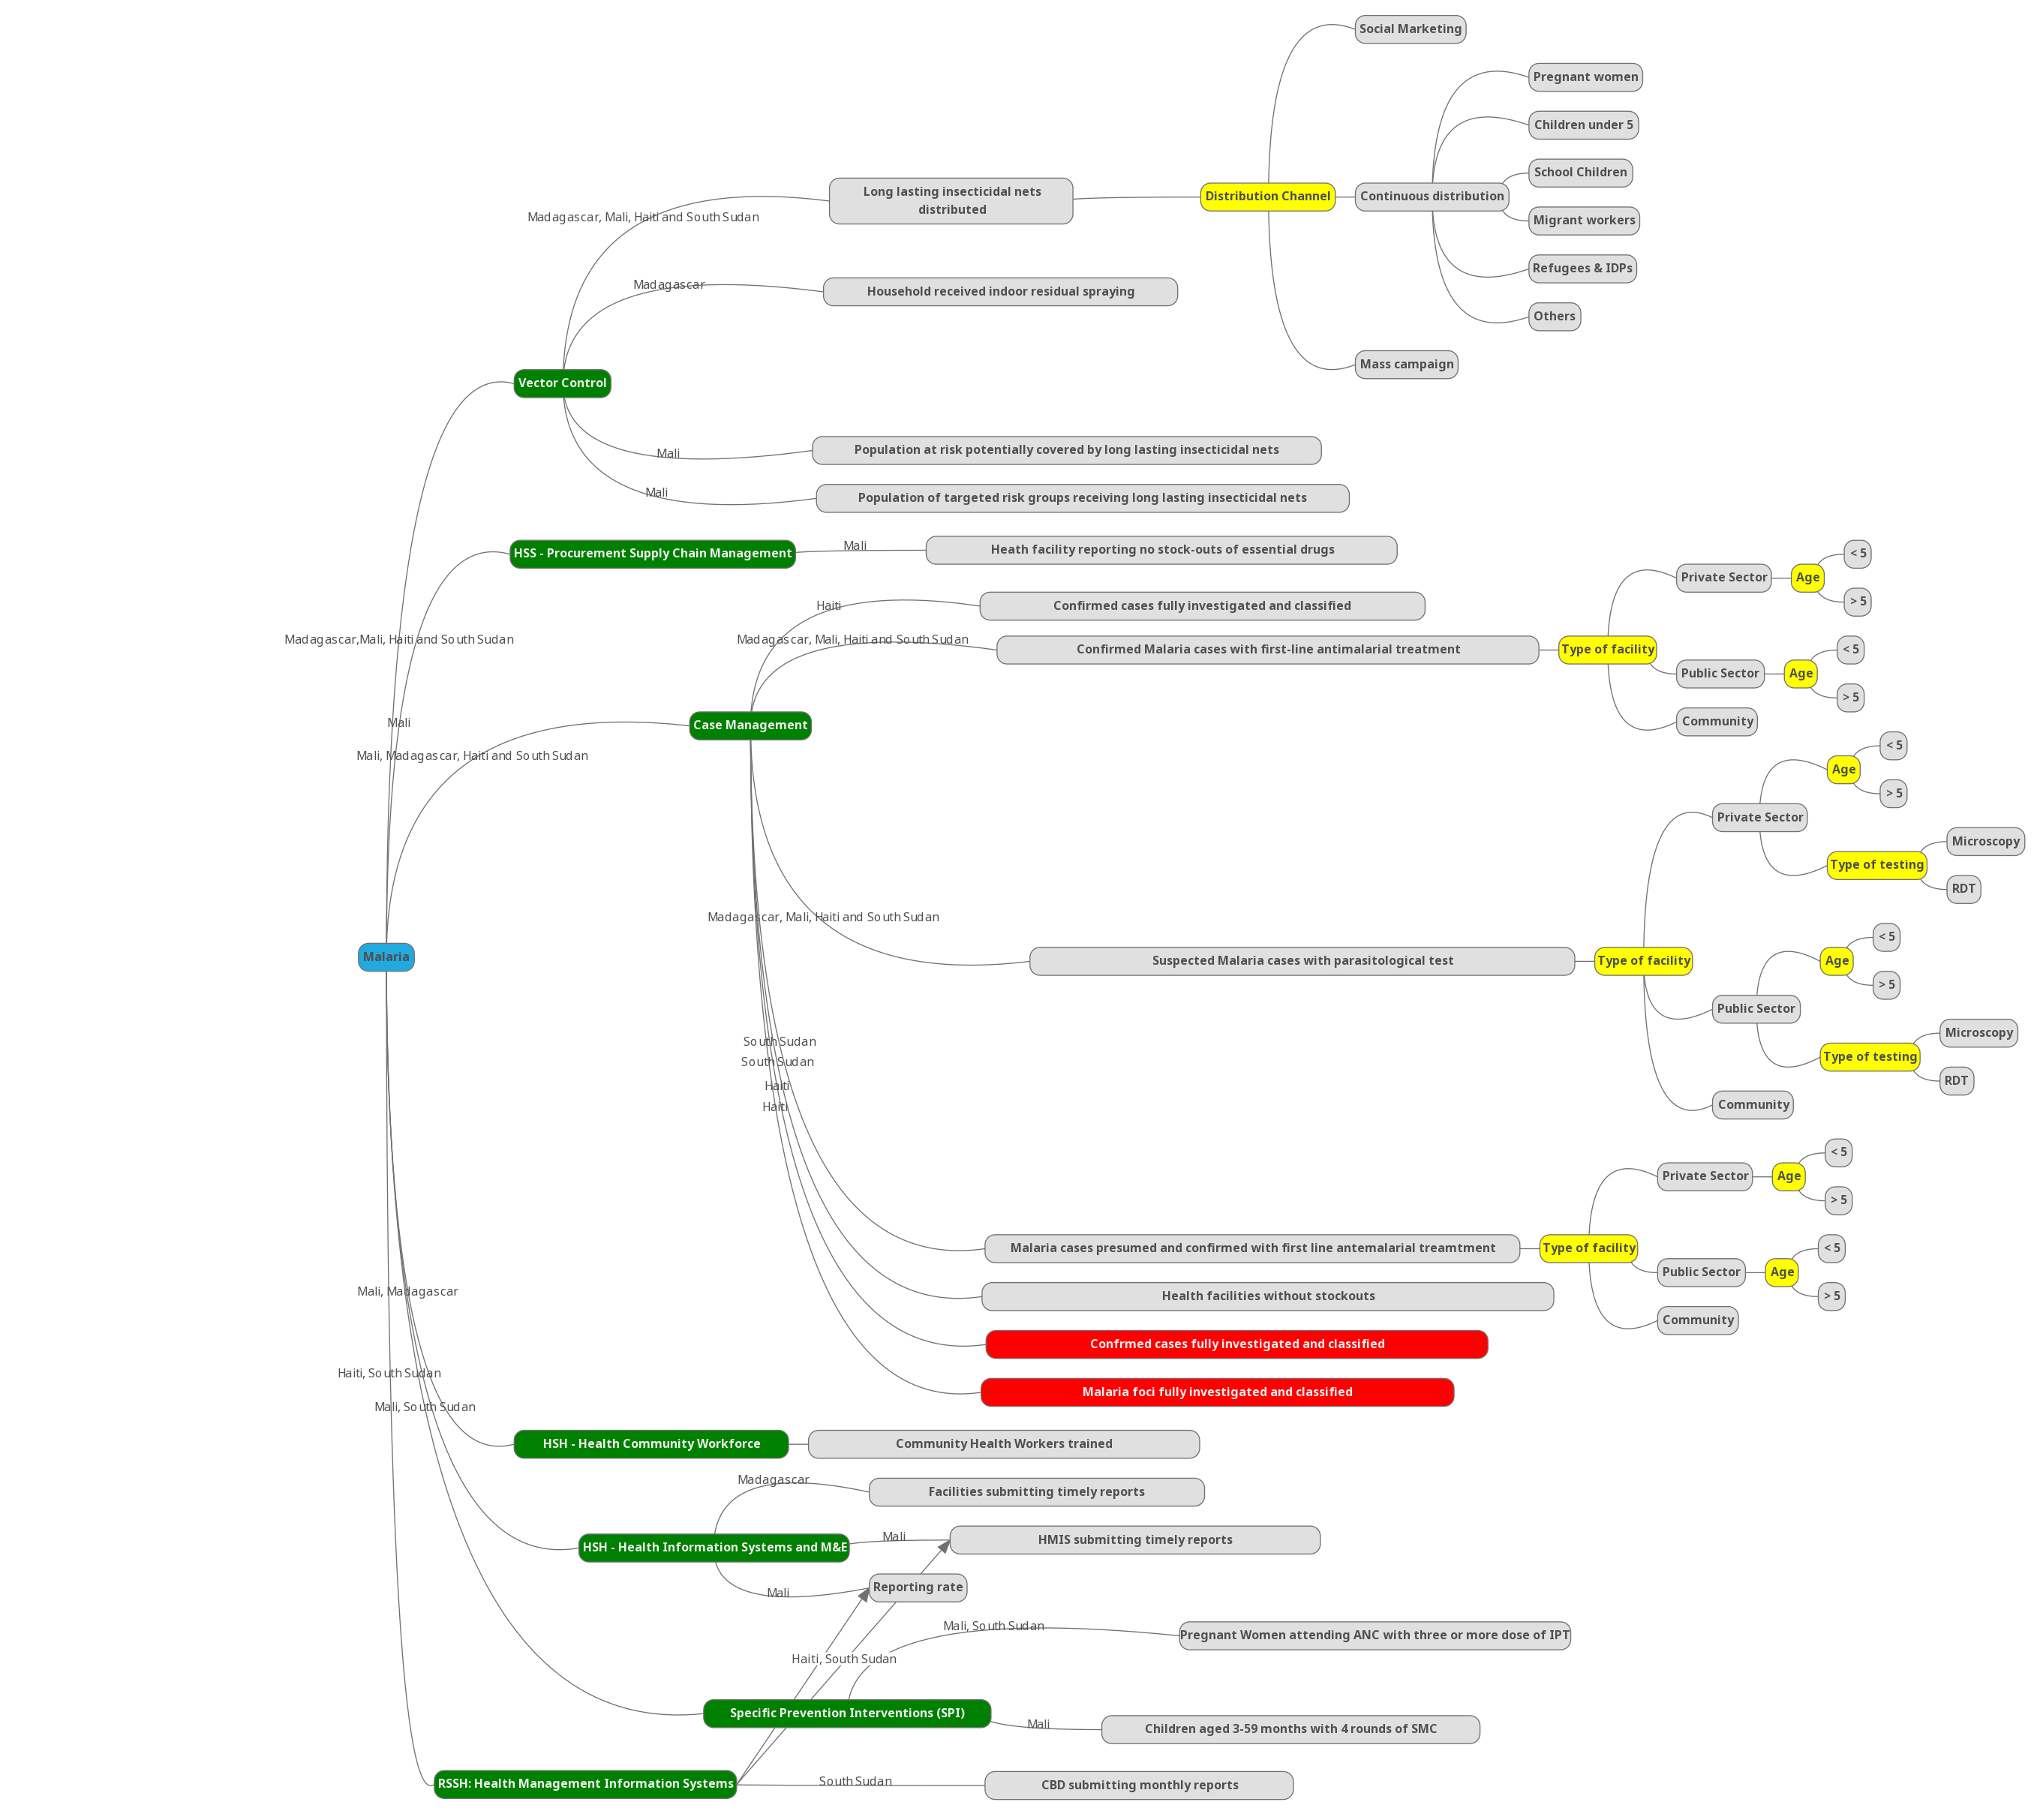
\includegraphics[width=0.8\linewidth]{./images/gfmublueprint-mal} 

}

\caption{Global Fund eTracker blueprint}\label{fig:nice-fig3}
\end{figure}

\hypertarget{indicator-tracking}{%
\chapter{Indicator Tracking}\label{indicator-tracking}}

Indicators are defined based on the GFMU reporting needs. However, countries may request for additional metrics, including country-level disaggregations based on the D2A framework. The indicators are aligned to global fund indicator matrix where modules group them and are classified by indicator codes. Each metric has a description which provides additional information on the analysis and interpretations.

Generally the GFMU tracks indicators in three main categories; baseline, targets and Achievement values as discussed below.

\begin{itemize}
\tightlist
\item
  \textbf{Baseline} - Provides the base measurement of the performance indicator before the implementation of the project
  activities. Its usually at the start of the reporting period.
\item
  \textbf{Targets} - A specific, planned level of result to be achieved within an explicit timeframe. Usually at the end of the reporting period. Targets are estimated based on the the Global Fund indicator classes.
\item
  \textbf{Achievement} - The actual measurement achieved in the reporting period. Usually at the end of the reporting period.
\end{itemize}

Below is an illustration of the indicator set up in Global Fund eTracker.

\begin{figure}

{\centering 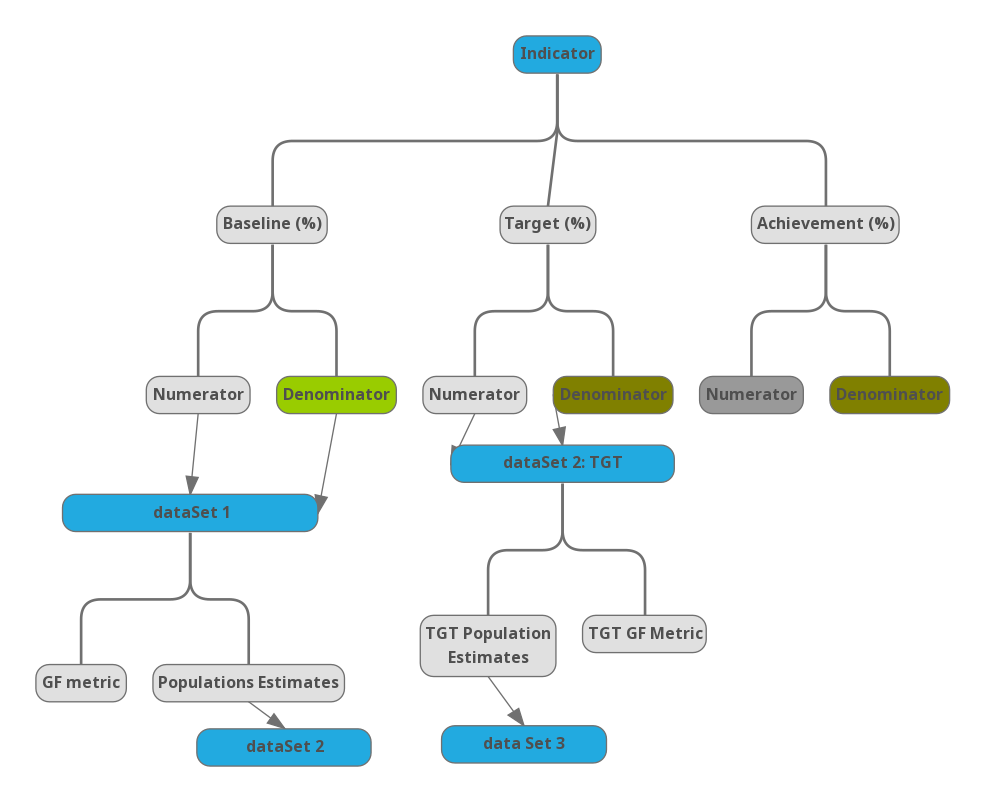
\includegraphics[width=0.8\linewidth]{./images/indicators} 

}

\caption{Global Fund eTracker Indicator Analysis}\label{fig:unnamed-chunk-2}
\end{figure}

\hypertarget{indicators}{%
\section{Indicators}\label{indicators}}

\label{tab:unnamed-chunk-3}Indicators

Code

Name of the Indicator

Description

HIV I-6

GF - Estimated child HIV infections

Description

This indicator is to assess the impact of antiretrovial medicine programmes on the number of children acquiring HIV by estimating the HIV transmission rate from women living with HIV to their children. The transmission can be calculated by using the Spectrum model.

In countries where data are available, facility attendance is high, and confirmatory tests are conducted systematically, efforts should be made to monitor the impact through directly assessing the percentage of children found to be HIV-positive among those born to HIV-positive mothers.

All countries should make efforts to monitor the HIV status and survival of children born to HIV-positive women, gathered during follow-up health care visits.

For further information refer to WHO publications on HIV monitoring and evaluation

Numerator:

Estimated children newly infected with HIV from mother-to-child transmission among children born in the previous 12 months to women living with HIV

Denominator

Estimated children delivered by women living with HIV who delivered in the previous 12 months

Source

Modelled (SPECTRUM MODEL)

Target type

Not applicable

Disaggregation of reported results

Not applicable

References

Same as in GARPR 2016 (Indicator 3.3)

Worded differently in:

WHO SI guide 2015- MTCT 7; Page 163- Percentage HIV-infected among HIV exposed infants born in the past 12 months

Global AIDS Monitoring2017- Indicator 2.2; Page 49- Estimated percentage of children newly infected with HIV from mother-to-child transmission among women living with HIV delivering in the past 12 months

HIV O-1(M)

GF - HIV+ve adults and children on treatment

Description

The reporting period is defined as any continuous 12-month period that has ended within a predefined number of months from the submission of the report. National reporting requirements can determine the predefined number of months. If the reporting period is 1 January to 31 December 2016, countries will calculate this indicator by using everyone who started antiretroviral therapy any time between 1 January and 31 December 2015.

Retention at 12 months after starting antiretroviral therapy is defined as the outcome. Those who have died since starting therapy, those who have stopped therapy and those lost to follow-up as of month 12 (or 24, 36, 48, 60, etc.) are included in the denominator but not in the numerator. For example, people who started antiretroviral therapy between 1 January and 31 December 2014 will have reached their 12-month outcomes for the reporting period 1 January to 31 December 2015.

As patients start antiretroviral therapy, monthly cohort data should be collected continuously for these patients. Data for monthly cohorts that have completed at least 12 months of treatment should then be aggregated. At facility level, patients who have transferrred out will not be counted either in the numerator or denominator. Patients who have transferred in will be counted in both numerator and denominator.

Survival over longer durations of treatment provide a better picture of the long-term effectiveness of ART. If this indicator is only produced in a sub-set of facilities, comment should be added on the source of information and whether the information is representative of all ART sites.

Numerator

PLHIV currently receiving antiretroviral therapy

Denominator

PLHIV and on antiretroviral therapy who have a suppressed viral load at 12 months (\textless{}1000 copies/ml)

Source

Program monitoring tools; ART registers and cohort and group analysis forms

Target type

Not applicable

Disaggregation of reported results

Sex (female, male)

Age (0-14; 15+)

Duration of treatment -24, 36 and 60 months

References

WHO SI guide 2015-ART-5; page 133;

Global AIDS Monitoring 2017- Indicator 1.3; Page 39; worded differently.
Percentage of adults and children living with HIV known to be on antiretroviral therapy 12 months after starting.

TB O-1a

GF - TB notification rate (All forms)

Description

It refers to all forms of TB cases that are bacteriologically confirmed or clinically diagnosed with active TB by a clinician.

It includes- new and relapse cases that are;

smear and/or culture positive; or smear positive/culture negative

smear and/or culture negative;

smear unknown/not done;

Positive by WHO-recommended rapid molecular diagnostics (e.g.~Xpert MTB/RIF);

extra-pulmonary cases confirmed by WRD;

cases confirmed on the basis of X-Ray abnormalities or suggestive histology;

It does not include- retreatment cases such as;

treatment after failure patients;

treatment after loss to follow-up (previously known as `treatment after default')

other retreatment cases

Numerator

Notified cases of all forms of TB-(i.E. Bacteriologically confirmed + clinically diagnosed) includes new and relapse cases

Denominator

Total Population

Source

TB register

Target type

Not applicable

Disaggregation of reported results

Not applicable

TCP-2 (M)

GF - TB Tx success rate

Description

Where applicable, report separately for all forms of TB cases provided
with treatment in prisons, or by a specific type of health care provider or the community.

This indicator is also reported as an coverage/output indicator to facilitate performance-based funding at each Progress Update and Disbursement Request (PU/DR).

For further details on all forms of TB cases included under this indicator please refer to comments above (cell P14) - below:

It includes- new and relapse cases that are;

smear and/or culture positive; or smear positive/culture negative

smear and/or culture negative;

smear unknown/not done;

Positive by WHO-recommended rapid molecular diagnostics (e.g.~Xpert MTB/RIF);

extra-pulmonary cases confirmed by WRD;

cases confirmed on the basis of X-Ray abnormalities or suggestive histology;

It does not include- retreatment cases such as;

treatment after failure patients;

treatment after loss to follow-up (previously known as `treatment after default')

other retreatment cases

Numerator

TB cases, all forms, bacteriologically confirmed plus clinically diagnosed, successfully treated (cured plus treatment completed) among all TB cases registered for treatment during, new and relapse cases

Denominator

Notified cases of all forms of TB-(i.E. Bacteriologically confirmed + clinically diagnosed) includes new and relapse cases

Source

Numerator:Number of all forms of TB cases who were successfully treated in each disaggregation cateogry

Denominator:Number of all forms of TB cases registered for treatment in each disaggregation category

Target type

Non cumulative (C)

Disaggregation of reported results

Sex (female, male)

Age (\textless{}15; 15+)

HIV status (positive, negative, not documented)

References

For details refer to indicator TB O-2a. Disaggregated data should be reported based on routine reporting, for example, in countries with electronic reporting systems or in a sample of randomly selected districts or sites

TB O-4 (M)

GF - RR TB and MDR-TB Tx success rate

Description

The period of assessment is 12 calendar months, usually counted from January to end December, and referred to as an annual cohort. All patients registered and starting treatment during this period are included in the calculation. In sites testing with Xpert MTB/RIF® alone, the indicator can be modified to include also RR-TB cases started on a full MDR-TB treatment regimen. Only laboratory confirmed RR-TB, MDR-TB and XDR-TB cases are counted for cohort reporting of Final Outcomes. It is measured 24 months after the end of the period of assessment. This gives sufficient time for most patients to complete their treatment and for the final culture results to be issued and recorded. All data can be extracted from the Second-line TB treatment register.

For example- Patients on a second-line drug regimen to be assessed are those who started on second-line drugs in the current calendar year minus three. Thus, if the current calendar year is 2017, the outcomes collated will be for the cohort started on second-line drugs in calendar year 2014. The report due date will be Q1 of 2018.

Numerator

Cases with RR-TB and/or MDR-TB began second-line treatment

Denominator

TB cases with RR-TB and/or MDR-TB notified

Source

Numerator:Number of bacteriologically-confirmed XDR-TB cases enrolled on second-line anti-TB treatment who are successfully treated

Denominator: Number bacteriologically-confirmed XDR-TB cases enrolled on second-line anti-TB treatment

Target type

Not applicable

Disaggregation of reported results

XDR TB

TB I-2

GF - TB incidence rate

Description

Refer to WHO TB report 2015 annex 1 for methods of measuring or estimating TB incidence in a given year.

In countries where the performance of TB surveillance systems do not allow the use notifications as a proxy for incidence, series of case notification rates should be carefully analyzed; and short-term forecasts may be used for planning and budgeting.

WHO recommends that all countries strengthen their surveillance systems until TB notifications are a direct measure (or close proxy) of TB incidence.

WHO also recommends that countries periodically assess TB incidence (its absolute values and trends) using a standard framework and tool for analyzing and documenting the reliability and coverage of TB notification data.

Numerator

Notified cases of all forms of TB-(i.E. Bacteriologically confirmed + clinically diagnosed) includes new and relapse cases

Denominator

Total Population

Source

TB recording and reporting system or Global TB report

Target type

Not applicable

Disaggregation of reported results

Not applicable

References

World Health Organization. Global taskforce on TB impact measurement

HIV O-4a (M)

GF - MSMs reporting condom use

Description

If data is available on another time period, include in the comments section.
If there are concerns that the data are not based on a representative sample, the interpretation of the survey data should reflect these concerns. Where different sources of data exist, the best available estimate should be used.

For further information refer to:
Operational guidelines for monitoring and evaluation of HIV programmes for sex workers, men who have sex with men, and transgender people. Chapel Hill (NC): MEASURE Evaluation; 2011

Numerator

MSMs reported condom used the last time they had anal sex with a male partner

Denominator

MSMs who reported having had anal sex with a male partner in the last six months

Source

Behavioural surveillance (BSS) or other special survey

Target type

Not applicable

Disaggregation of reported results

Age (\textless{}25 and \textgreater{}25)

References

WHO SI guide 2015-PREV.1.b; page 75;

Global AIDS Monitoring 2017- Indicator 3.6B; Page 68

HIV O-5 (M)

GF - Sex workers reporting condom use

Description

This indicator asks about commercial sex in the past 12 months. If data is available on another time period, such as last three or 12 months, include in the comments section.

If there are concerns that the data are not based on a representative sample, the interpretation of the survey data should reflect these concerns. Where different sources of data exist, the best available estimate should be used.

Numerator

Sex workers reported condom used with their last client

Denominator

Sex workers who reported having commercial sex in the last 12 months

Source

Behavioural surveillance (BSS) or other special survey

Target type

Not applicable

Disaggregation of reported results

Sex (female, male)

Age (\textless{}25 and \textgreater{}25)

References

For further information refer to:

Operational guidelines for monitoring and evaluation of HIV programmes for sex workers, men who have sex with men, and transgender people. Chapel Hill (NC): MEASURE Evaluation; 2011

WHO SI guide 2015-PREV.1.b; page 75;

Global AIDS Monitoring 2017- Indicator 3.6A; Page 66

KP-1a (M)

GF - MSMs with HIV prevention programs

Description

These indicators aim to monitor coverage of HIV prevention programs using program data and population size estimates. Where size estimations are not available, countries will be required to undertake estimation exercise as soon as possible. Until the revised estimates are provided, available estimates will be used as denominators.

Data is generated by counting people who receive a defined package of services that includes the minimum specified components- BCC; provision of consumables (condoms; lubricants, needles and syringes as needed); referral to another service such as STI diagnosis and treatment, HIV testing and counseling, etc. In addition, it could include other interventions from the comprehensive package of services.

The components of the package of HIV prevention interventions should be defined at country level and tailored to the needs of the target population. Refer to the comprehensive package of services recommended by technical partners-
Tool to set and monitor targets for HIV prevention, diagnosis, treatment and care for key populations: supplement to the 2014 consolidated guidelines for HIV prevention, diagnosis, treatment and care for key populations. Geneva:
World Health Organization; 2015

Data collection requires reliable tracking systems that are designed to count the number of individual ``clients served'' at the same service or across services as opposed to the ``client visits''. This can be ensured through implementation of Unique Identification Codes (UIC). In the absence of UIC, report on the number of contacts until the time when a system to avoid double counting is set up. Agree on a timeframe for setting up such system and ensure adequate funds are available.

The coverage data from routine reporting will be triangulated with the coverage from survey data for overall impact assessment.

When targeting ``other vulnerable populations'' specify in the comments column of the performance framework which populations are being targeted.

Numerator

MSMs reached with HIV prevention programs defined package of services

Denominator

Estimated MSMs

Source

Numerator: Program records

Denominator: Estimated population size

Target type

Non cumulative (A/ B/ E ) or Cumulative annually (D)

Disaggregation of reported results

Not applicable

KP-1a (M)b

GF - TGT MSMs with HIV prevention programs

Description

These indicators aim to monitor coverage of HIV prevention programs using program data and population size estimates. Where size estimations are not available, countries will be required to undertake estimation exercise as soon as possible. Until the revised estimates are provided, available estimates will be used as denominators.

Data is generated by counting people who receive a defined package of services that includes the minimum specified components- BCC; provision of consumables (condoms; lubricants, needles and syringes as needed); referral to another service such as STI diagnosis and treatment, HIV testing and counseling, etc. In addition, it could include other interventions from the comprehensive package of services.

The components of the package of HIV prevention interventions should be defined at country level and tailored to the needs of the target population. Refer to the comprehensive package of services recommended by technical partners-
Tool to set and monitor targets for HIV prevention, diagnosis, treatment and care for key populations: supplement to the 2014 consolidated guidelines for HIV prevention, diagnosis, treatment and care for key populations. Geneva:
World Health Organization; 2015

Data collection requires reliable tracking systems that are designed to count the number of individual ``clients served'' at the same service or across services as opposed to the ``client visits''. This can be ensured through implementation of Unique Identification Codes (UIC). In the absence of UIC, report on the number of contacts until the time when a system to avoid double counting is set up. Agree on a timeframe for setting up such system and ensure adequate funds are available.

The coverage data from routine reporting will be triangulated with the coverage from survey data for overall impact assessment.

When targeting ``other vulnerable populations'' specify in the comments column of the performance framework which populations are being targeted.

Numerator

TGT MSMs reached with HIV prevention programs defined package of services

Denominator

TGT Estimated MSMs

Source

Numerator: Program records

Denominator: Estimated population size

Target type

Non cumulative (A/ B/ E ) or Cumulative annually (D)

Disaggregation of reported results

Not applicable

KP-1c (M)

GF - Sex workers with HIV programs

KP-1c (M)b

GF - TGT sex workers with HIV programs

KP-3c (M)

GF - Sex workers with HIV result

Description

Coverage will be assessed based on population size estimates. Where these are not available, countries will be required to undertake a size estimation as soon as possible. Until the revised estimates are provided, available, estimates will be used.

Coverage data from routine reporting will be triangulated with the coverage from survey data for overall impact assessment.

If data on persons who retest are not available, this indicator (reported as numbers only) will give information on the number of times HIV testing and counseling services were delivered, rather than the number of individuals who received HIV testing and counseling services.

Numerator

Sex workers received an HIV test and know their results

Denominator

Estimated sex workers

Source

Numerator: Program records

Denominator:Estimated population size

Target type

Non cumulative (A/ B/ E ) or Cumulative annually (D)

Disaggregation of reported results

Not applicable

References

WHO SI guide 2015: HTS 7; page 100

Global AIDS Monitoring 2017- Indicator 3.4; Page 62; Different indicator.
Knowledge of HIV status among sex workers

KP-3c (M)b

GF - TGT Sex workers with HIV result

Description

Coverage will be assessed based on population size estimates. Where these are not available, countries will be required to undertake a size estimation as soon as possible. Until the revised estimates are provided, available, estimates will be used.

Coverage data from routine reporting will be triangulated with the coverage from survey data for overall impact assessment.

If data on persons who retest are not available, this indicator (reported as numbers only) will give information on the number of times HIV testing and counseling services were delivered, rather than the number of individuals who received HIV testing and counseling services.

Numerator

TGT Sex workers received an HIV test and know their results

Denominator

TGT Estimated sex workers

Source

Numerator: Program records

Denominator:Estimated population size

Target type

Non cumulative (A/ B/ E ) or Cumulative annually (D)

Disaggregation of reported results

Not applicable

References

WHO SI guide 2015: HTS 7; page 100

Global AIDS Monitoring 2017- Indicator 3.4; Page 62; Different indicator.
Knowledge of HIV status among sex workers

Kp-1e

GF - Vulnerable population with HIV programs

Kp-1eb

GF - TGT Vulnerable population with HIV programs

KP-3e

GF - Vulnerable population with HIV results

Description

Coverage will be assessed based on population size estimates. Where these are not available, countries will be required to undertake a size estimation as soon as possible. Until the revised estimates are provided, available, estimates will be used.

Coverage data from routine reporting will be triangulated with the coverage from survey data for overall impact assessment.

If data on persons who retest are not available, this indicator (reported as numbers only) will give information on the number of times HIV testing and counseling services were delivered, rather than the number of individuals who received HIV testing and counseling services.

When targeting ``other vulnerable populations'' specify in the comments column of the performance framework which populations are being targeted.

Numerator

Other vulnerable populations received an HIV test and know their results

Denominator

Estimated other vulnerable populations

Source

Numerator: Program records

Denominator: Estimated population size

Target type

Non cumulative (A/ B/ E ) or Cumulative annually (D)

Disaggregation of reported results

Not applicable

References

WHO SI guide 2015: HTS 7; page 100

Kp-3eb

GF - TGT Vulnerable population with HIV results

Description

Coverage will be assessed based on population size estimates. Where these are not available, countries will be required to undertake a size estimation as soon as possible. Until the revised estimates are provided, available, estimates will be used.

Coverage data from routine reporting will be triangulated with the coverage from survey data for overall impact assessment.

If data on persons who retest are not available, this indicator (reported as numbers only) will give information on the number of times HIV testing and counseling services were delivered, rather than the number of individuals who received HIV testing and counseling services.

When targeting ``other vulnerable populations'' specify in the comments column of the performance framework which populations are being targeted.

Numerator

TGT Other vulnerable populations received an HIV test and know their results

Denominator

TGT Estimated other vulnerable populations

Source

Numerator: Program records

Denominator: Estimated population size

Target type

Non cumulative (A/ B/ E ) or Cumulative annually (D)

Disaggregation of reported results

Not applicable

References

WHO SI guide 2015: HTS 7; page 100

PMTCT-1

GF - Pregnant Women with HIV results

Description

Coverage will be assessed based on population size estimates.

Population based survey data (for example, DHS or AIDS Indicator Survey), when available, will be used for triangulation purposes.

This indicator enables countries to monitor trends over time in HIV testing among pregnant women. Disaggregated data by regions may allow to identify lower performing areas.

While it is not feasible to avoid double counting entirely, countries should ensure data collection and reporting system is in place to miniumize it, such as using patient held and facility held ANC records to doucment that testing took place

Include those with previously known HIV infection in the numerator- even if they do not receive an HIV test, their HIV infection is identified for susequent PMTCT interventions

Numerator

Pregnant women who know their HIV status

Denominator

Estimated pregnant women who delivered within the past 12 months

Source

Numerator: Program records, e.g.~ANC registers, labour and delivery registers.

Denominator: Estimates from central statistics office, UN Population Division
or vital statistics.

Target type

Non cumulative (B) or Cumulative annually (D)

Disaggregation of reported results

Not applicable

References

WHO SI guide 2015: HTS.4 (page 99) and MTCT.1; Page 160

PMTCT-1b

GF - TGT Pregnant Women with HIV results

Description

Coverage will be assessed based on population size estimates.

Population based survey data (for example, DHS or AIDS Indicator Survey), when available, will be used for triangulation purposes.

This indicator enables countries to monitor trends over time in HIV testing among pregnant women. Disaggregated data by regions may allow to identify lower performing areas.

While it is not feasible to avoid double counting entirely, countries should ensure data collection and reporting system is in place to miniumize it, such as using patient held and facility held ANC records to doucment that testing took place

Include those with previously known HIV infection in the numerator- even if they do not receive an HIV test, their HIV infection is identified for susequent PMTCT interventions

Numerator

TGT Pregnant women who know their HIV status

Denominator

TGT Estimated pregnant women who delivered within the past 12 months

Source

Numerator: Program records, e.g.~ANC registers, labour and delivery registers.

Denominator: Estimates from central statistics office, UN Population Division
or vital statistics.

Target type

Non cumulative (B) or Cumulative annually (D)

Disaggregation of reported results

Not applicable

References

WHO SI guide 2015: HTS.4 (page 99) and MTCT.1; Page 160

PMTCT-2.1

GF - HIV +ve pregnant women on ART

Description

Countries are encouraged to track and report the number of women receiving the various regimens so that the impact of antiretroviral medicines on mother-to-child transmission can be modelled based on their efficacy. If countries do not have a system for collecting and reporting this data, they should establish one. Efforts should be made to remove women captured twice in the reporting systems.

To ensure comparability, the Spectrum output is used for the denominator for global analysis.

Numerator

HIV + pregnant women who received art during pregnancy

Denominator

Estimated HIV positive pregnant women who delivered

Source

Numerator: Program records, e.g.~PMTCT registers, ARV registers.

Denominator:Estimation models such as Spectrum or antenatal clinic surveillance surveys combined with demographic data and appropriate adjustments related to the coverage of antenatal clinic surveys.

Target type

Non cumulative (B) or Cumulative annually (D)

Disaggregation of reported results

Not applicable

References

WHO SI guide 2015: MTCT.2; page 161

Global AIDS Monitoring 2017- Indicator 2.3; Page 51; worded differently.
\% of HIV positive pregnant women living with HIV who received anti-retroviral medicines to reduce the risk of mother to child transmission

PMTCT-2.1b

GF - TGT HIV +ve pregnant women on ART

Description

Countries are encouraged to track and report the number of women receiving the various regimens so that the impact of antiretroviral medicines on mother-to-child transmission can be modelled based on their efficacy. If countries do not have a system for collecting and reporting this data, they should establish one. Efforts should be made to remove women captured twice in the reporting systems.

To ensure comparability, the Spectrum output is used for the denominator for global analysis.

Numerator

TGT HIV + pregnant women who received art during pregnancy

Denominator

TGT Estimated HIV positive pregnant women who delivered

Source

Numerator: Program records, e.g.~PMTCT registers, ARV registers.

Denominator:Estimation models such as Spectrum or antenatal clinic surveillance surveys combined with demographic data and appropriate adjustments related to the coverage of antenatal clinic surveys.

Target type

Non cumulative (B) or Cumulative annually (D)

Disaggregation of reported results

Not applicable

References

WHO SI guide 2015: MTCT.2; page 161

Global AIDS Monitoring 2017- Indicator 2.3; Page 51; worded differently.
\% of HIV positive pregnant women living with HIV who received anti-retroviral medicines to reduce the risk of mother to child transmission

TCS-1 (M)

GF - PLHIV on ART

Description

The count should not include people who have stopped treatment, died or emigrated to another country or who are otherwise lost to follow-up at the facility during this period. Protocols should be in place to avoid duplicate counting of individuals across facilities or over time.

This indicator does not include antiretroviral medicines taken only for preventing mother-to-child transmission and post-exposure prophylaxis. This
indicator includes pregnant women living with HIV who are receiving lifelong antiretroviral therapy.

Countries should triangulate the numerator from programme data with national procurement and drug monitoring systems and adjust reported numbers as appropriate.

Countries that undertake data quality assessments or reviews that monitor the extent to which facilities are able to accurately report the number of people on treatment during reporting periods should also adjust programme numerator data to account for these inconsistencies.

Estimates of coverage of antiretroviral therapy from surveys can also be used to inform or validate the numerator. Note that surveys that only capture self-reported data on treatment uptake should not be used, since self-reported data has been shown to be of limited quality.

Numerator

PLHIV currently receiving antiretroviral therapy

Denominator

Estimated PLHIV

Source

Numerator: Program records, e.g.~ART registers and corresponding cross-sectional reporting forms.

Denominator: HIV estimation models such as Spectrum

Target type

Non cumulative E

Disaggregation of reported results

Sex (female, male)

Age (\textless{}15, 15+)

Age \textbar{} Gender 15-19 (female, male)*

Age \textbar{} Gender 20-24 (female, male)*

Age \textbar{} Gender 15-24 (female, male)*●

KPs: MSM, TG people, Sex Workers, PWIDs

*To be reported from selected countries

●To be reported in cases where data for age groups 15-19 and 20-24 is not available

References

WHO SI guide 2015: ART.3; page 132

Global AIDS monitoring 2017- indicator 1.2; Page- 37; worded differently.
Percentage and number of adults and children on antiretroviral therapy among all adults and children living with HIV at the end of the reporting period

TCS-1 (M)b

GF - TGT PLHIV on ART

Description

The count should not include people who have stopped treatment, died or emigrated to another country or who are otherwise lost to follow-up at the facility during this period. Protocols should be in place to avoid duplicate counting of individuals across facilities or over time.

This indicator does not include antiretroviral medicines taken only for preventing mother-to-child transmission and post-exposure prophylaxis. This
indicator includes pregnant women living with HIV who are receiving lifelong antiretroviral therapy.

Countries should triangulate the numerator from programme data with national procurement and drug monitoring systems and adjust reported numbers as appropriate.

Countries that undertake data quality assessments or reviews that monitor the extent to which facilities are able to accurately report the number of people on treatment during reporting periods should also adjust programme numerator data to account for these inconsistencies.

Estimates of coverage of antiretroviral therapy from surveys can also be used to inform or validate the numerator. Note that surveys that only capture self-reported data on treatment uptake should not be used, since self-reported data has been shown to be of limited quality.

Numerator

TGT PLHIV currently receiving antiretroviral therapy

Denominator

TGT Estimated PLHIV

Source

Numerator: Program records, e.g.~ART registers and corresponding cross-sectional reporting forms.

Denominator: HIV estimation models such as Spectrum

Target type

Non cumulative E

Disaggregation of reported results

Sex (female, male)

Age (\textless{}15, 15+)

Age \textbar{} Gender 15-19 (female, male)*

Age \textbar{} Gender 20-24 (female, male)*

Age \textbar{} Gender 15-24 (female, male)*●

KPs: MSM, TG people, Sex Workers, PWIDs

*To be reported from selected countries

●To be reported in cases where data for age groups 15-19 and 20-24 is not available

References

WHO SI guide 2015: ART.3; page 132

Global AIDS monitoring 2017- indicator 1.2; Page- 37; worded differently.
Percentage and number of adults and children on antiretroviral therapy among all adults and children living with HIV at the end of the reporting period

TCP-3

GF - Labs with adq. performance of SMs

Description

External quality assurance for smear microscopy is performed by rechecking slides. No error of any type is considered a target for optimal performance. Any major error (high false-positive or high false-negative) may indicate unacceptable performance.

Numerator

Laboratories showing adequate performance in external quality assurance for smear microscopy among the total laboratories undertake smear microscopy

Denominator

Total laboratories undertaking smear microscopy

Source

Numerator: NTP administration records

Denominator: NTP administration records

Target type

Non cumulative (B)

Disaggregation of reported results

Not applicable

TCP-5

GF - Under 5 incontact with TB patients

Description

Numerator:

Children \textless{}5 in contact with TB patients who began isonizide preventive therapy

Denominator

Not applicable

Source

Numerator: Program records

Denominator: Not applicable

Target type

Non cumulative (A)

Disaggregation of reported results

Not applicable

TCP 6a

GF - TB cases (all forms) notifed to prisoners

Description

Numerator

Denominator

Source

TB register at the basic management unit, community health unit

Target type

Not applicable

Disaggregation of reported results

Not applicable

TB/HIV-3.1

GF - PLHIV screened for TB

Description

Indicator measurement same as before, wording revised by partners.

Intensified TB case finding should be implemented at all HIV care and treatment facilities and TB status of people living with HIV should be assessed at every visit during the reporting period. It is also important to monitor implementation of the entire cascade of care, starting from symptom screening to diagnosis and treatment of TB. This necessitates close coordination between the NACP and NTP but responsibility of reporting lies with the NACP

Numerator

PLHIV in care (including pmtct) who are screened for TB in HIV care or treatment settings

Denominator

PLHIV currently receiving antiretroviral therapy

Source

Numerator: pre-ART and ART register and cross-sectional quarterly reports

Denominator: pre-ART and ART register and cross-sectional quarterly reports

Target type

Non cumulative (C)

Disaggregation of reported results

Not applicable

References

WHO SI guide 2015: LINK.18; page 119

A guide to monitoring and evaluation for collaborative TB/HIV activities: 2015 revision- Indicator B.1; Page 22-

TB/HIV-6 (M)

GF - HIV+ve new and relapse TB patients on ART

Description

Prompt TB treatment and early ART are critical for reducing the mortality due to HIV-associated TB and must be the highest-priority activity for both the NACP and NTP. While TB treatment should be started immediately, ART should be started within 8 weeks of TB diagnosis, given that all are eligible for ART irrespective of their CD4 cell count.

Although it is important that ART status of all HIV positive TB patients is assessed, this indicator considers only new and relapse patients to avoid double counting. Cases with undocumented TB treatment history should be counted as new cases.

TB and HIV programmes should aim to achieve TB treatment and ART in more than 90\% of HIV positive TB patients. However, this indicator may miss patients diagnosed towards the end of reporting period whose ART treatment status may not be updated in the TB registers. Also, this indicator does not capture timeliness of ART initiation.

Numerator

HIV + new and relapse TB patients on art during TB treatment

Denominator

HIV + new and relapsed TB patients registered .

Source

Numerator and
Denominator: TB register at the basic management unit, Pre-ART register and ART register.

Target type

Non cumulative (C)

Disaggregation of reported results

Not applicable

References

WHO SI 2015 guidelines: LINK.16; page 118

A guide to monitoring and evaluation for collaborative TB/HIV activities: 2015 revision- Indicator A.4; Page 18-

MDR-TB 2 (M)

GF - RR-TB and MDR-TB cases notified

Description

To be computed separately for patients detected with rifampicin resistant TB (RR-TB) alone in sites using Xpert MTB/RIF

Numerator

TB cases with RR-TB and/or MDR-TB notified

Denominator

Not applicable

Source

Numerator: Lab register for culture, DST and xpert

Denominator: Not applicable

Target type

Non cumulative (A)

Disaggregation of reported results

Sex (female, male)

Age (\textless{}15; 15+)

References

'Companion handbook to the WHO guidelines for the programmatic management of drug-resistant tuberculosis: WHO, 2014. Annex 5, page 407;

MDR-TB 2 (M)b

GF - TGT RR-TB and MDR-TB cases notified

Description

To be computed separately for patients detected with rifampicin resistant TB (RR-TB) alone in sites using Xpert MTB/RIF

Numerator

TGT TB cases with RR-TB and/or MDR-TB notified

Denominator

Not applicable

Source

Numerator: Lab register for culture, DST and xpert

Denominator: Not applicable

Target type

Non cumulative (A)

Disaggregation of reported results

Sex (female, male)

Age (\textless{}15; 15+)

References

'Companion handbook to the WHO guidelines for the programmatic management of drug-resistant tuberculosis: WHO, 2014. Annex 5, page 407;

MDR-TB 3 (M)

GF - RR-TB and MDR-TB cases on second-line Tx

Confirmed cases fully investigated \& class.

MDR-TB 3 (M)b

GF - TGT RR-TB and MDR-TB cases on second-line Tx

Description

The programme manager is responsible to ensure that all patients in whom RR-TB or MDR-TB is detected are placed on appropriate treatment in the shortest time possible. This may also apply to patients at risk of infection with RR-TB but who are not confirmed (presumptive).

Patients detected with rifampicin-resistant TB (RR-TB) in sites using Xpert MTB/RIF to be included in the denominator as well as numerator.

A comparison of enrolled to identified RR-TB/MDR-TB cases gives an indication of access to care although patients started on treatment may have been detected prior to the period of assessment. Comparator data are sourced from the Laboratory register for culture, Xpert MTB/RIF® and DST (using the date of DST result).

The suggested period of assessment is six calendar months, the first usually counted from January to end June and July to end December. Indicators are measured in the month following the end of the six-month period.

Numerator

TGT cases with RR-TB and/or MDR-TB began second-line treatment

Denominator

Not applicable

Source

Numerator: Second line TB treatment register

Denominator: Not applicable

Target type

Non cumulative (A)

Disaggregation of reported results

Sex (female, male)

Age (\textless{}15; 15+)

New TB drugs;Short regimens

MDR-TB 4

GF - RR-TB and MDR-TB cases on treatement lost to follow up

Description

Patients with rifampicin- resistant TB (RR-TB) in sites using Xpert MTB/ RIF who are on treatment to be included in the denominator as well as numerator
Lost to follow up refers to treatment interruption for two or more consecutive months for any reason without medical approval.

Treatment for MDR-TB may take 9 months (short regimens) to 20 months or more and final outcomes can thus only be assessed one to three years after the start of enrolment. The programme manager often needs an indication of how patients are faring, well before that. This is particularly important when a drug-resistant TB treatment programme is starting. Once a program ``matures,'' the final outcomes become more useful to monitor.

All lab confirmed RR-TB and MDR-TB patients registered and starting treatment during the period of assessment are counted for reporting of Interim Results. The denominator also includes XDR-TB cases started on prescribed treatment with second-line drugs
The suggested period of assessment is six calendar months. This is usually counted from January to end June and July to end December. Indicators are measured three months after the end of the six-month period. There will be a six month timelag in reporting results from the end of a six monthly cohort.

Numerator

Cases with RR-TB and/or MDR-TB started on treatment for MDR-TB lost to follow up during the first six months of treatment

Denominator

Cases with RR-TB and/or MDR-TB began second-line treatment

Source

Numerator: Second line TB treatment register

Denominator: Second line TB treatment register

Target type

Non cumulative (C)

Disaggregation of reported results

M\&E-1

GF - Reporting units submitting timely reports

Description

Numerator

HMIS or other routine reporting units submitting timely reports according to national guidelines

Denominator

Total HMIS or other routine reporting units

Source

Numerator: HMIS, program records

Denominator: HMIS, program records

Target type

Non cumulative
(B)

Disaggregation of reported results

References

HSS

TCS-3.1

GF - PLHIV and on ART with suppressed VL

Description

The +/- 3 months allows to know if someone is still ``on ART''. For example, for the cohort of people on ART in 2015, one would need to wait until March 2016 to know for sure if they are on ART because if they were supposed to come in December, but they are late and come within 3 months from their appointment, they are still counted to be on ART. But in March (3 months after their Dec appointment), if they do not come, then they are counted as not on ART in Dec 2015. In Dec 2015, one would know for sure about the cohort that started in Sept 2014. The +/- 3months period allows for accommodating reporting practices that may vary from country to country- some countries report based on the Sept cohort and others try to wait until March; and some others report end Dec for the full calendar cohort, and just make assumptions that everyone is on ART (no drop out for the Nov/Dec cohort you may not have information on yet) at the time of reporting.

As an EWI of HIVDR, it reflects ability of facility to attain a level of care that avoids HIVDR. Good performance is \textgreater{}85\%; passable performance is \textgreater{}70\%.

Numerator

PLHIV and on antiretroviral therapy who have a suppressed viral load at 12 months (\textless{}1000 copies/ml)

Denominator

PLHIV who intiated art 12 months (±3 months) before the start of the reporting period

Source

Numerator: Number of PLHIV who initiated ART 12 months (±3 months) before the start of the reporting period and who have a suppressed viral load (\textless{}1000 copies/ml) at 12 months after initiating ART in each disaggregation category

Denominator: Number ofpeople living with HIV who intiated ART 12 months (±3 months) before the start of the reporting period in each disaggregation category.

Target type

Not applicable

Disaggregation of reported results

CM-1a(M)

GF - Suspected Malaria tested

Description

For countries that maintain a record of suspected cases, use the `number of suspected cases' as denominator

Where countries do not keep record of suspected cases, the following method used for World Malaria Report data, will be used to calculate suspected cases

Suspected cases= cases tested + presumed cases⃰ reported⃰

Presumed cases= total reported cases -- confirmed cases.

In cases where reported cases are not differentiated as confirmed and presumed, the positive cases from lab register can be used a proxy for confirmed cases.
The latter assumes that all those confirmed as malaria were treated.

Numerator

Suspected malaria cases received a parasitological test

Denominator

All suspected malaria cases present

Source

Numerator: Lab register or records of RDT use

Denominator: Suspect register/ OPD register/ Treatment register

Target type

Non cumulative (C)

Disaggregation of reported results

Age (\textless{}5, \textgreater{}5)

Type of testing (Microscopy, RDT)

CM-1a(M)b

GF - TGT Suspected Malaria tested

Description

For countries that maintain a record of suspected cases, use the `number of suspected cases' as denominator

Where countries do not keep record of suspected cases, the following method used for World Malaria Report data, will be used to calculate suspected cases

Suspected cases= cases tested + presumed cases⃰ reported⃰

Presumed cases= total reported cases -- confirmed cases.

In cases where reported cases are not differentiated as confirmed and presumed, the positive cases from lab register can be used a proxy for confirmed cases.
The latter assumes that all those confirmed as malaria were treated.

Numerator

TGT Suspected malaria cases received a parasitological test

Denominator

TGT All suspected malaria cases present

Source

Numerator: Lab register or records of RDT use

Denominator: Suspect register/ OPD register/ Treatment register

Target type

Non cumulative (C)

Disaggregation of reported results

Age (\textless{}5, \textgreater{}5)

Type of testing (Microscopy, RDT)

CM-2a (M)

GF - Confirmed Malaria treated

Description

Performance assessment will be based on trends in malaria cases in the country

Numerator

Confirmed malaria cases received first-line antimalarial treatment according to national policy

Denominator

Confirmed malaria cases present

Source

Numerator: OPD register/
Malaria treatment register/
Pharmacy

Denominator: Lab registers

Target type

Non cumulative (C)

Disaggregation of reported results

Age (\textless{}5, \textgreater{}5 year)

CM-2a (M)b

GF - TGT Confirmed Malaria treated

Description

Performance assessment will be based on trends in malaria cases in the country

Numerator

TGT confirmed malaria cases received first-line antimalarial treatment according to national policy

Denominator

TGT confirmed malaria cases present

Source

Numerator: OPD register/
Malaria treatment register/
Pharmacy

Denominator: Lab registers

Target type

Non cumulative (C)

Disaggregation of reported results

Age (\textless{}5, \textgreater{}5 year)

CM-5 (M)

GF - Confirmed cases fully investigated and classifed

Description

Including case investigation form, focus investigation form and active case detection.

Numerator

Confirmed cases fully investigated and classified

Denominator

Confirmed malaria cases present

Source

Malaria case investigation database

Target type

Non cumulative (C)

Disaggregation of reported results

References

Disease surveillance for malaria elimination- an operational manual, WHO, June 2013

CM-5 (M)b

GF - TGT confirmed cases fully investigated and classifed

Description

Including case investigation form, focus investigation form and active case detection.

Numerator

TGT confirmed cases fully investigated and classified

Denominator

TGT confirmed malaria cases present

Source

Malaria case investigation database

Target type

Non cumulative (C)

Disaggregation of reported results

References

Disease surveillance for malaria elimination- an operational manual, WHO, June 2013

CM-6 (M)

GF - Malaria foci fully investigated and classified

Description

Malaria focus investigation form completed, including data from an entomological investigation and registered (on register, with maps of each focus) (\# \& \%)

Numerator

Malaria foci fully investigated and classified

Denominator

TGT confirmed malaria cases present

Source

Malaria case investigation database

Target type

Non cumulative (C)

Disaggregation of reported results

References

Disease surveillance for malaria elimination- an operational manual, WHO, June 2013

CM-6 (M)b

GF - TGT Malaria foci fully investigated and classified

Description

Malaria focus investigation form completed, including data from an entomological investigation and registered (on register, with maps of each focus) (\# \& \%)

Numerator

TGT malaria foci fully investigated and classified

Denominator

TGT confirmed malaria cases present

Source

Malaria case investigation database

Target type

Non cumulative (C)

Disaggregation of reported results

References

Disease surveillance for malaria elimination- an operational manual, WHO, June 2013

VC-3 (M)

GF - LLINs distributed continously

Description

Specify in the comments column of the performance framework which group(s) are being targeted

Numerator

Long-lasting insecticidal nets distributed to targeted risk groups - through continuous distribution

Denominator

Not applicable

Source

Program records of ITN distribution at specific sites

Target type

Non cumulative (A)

Disaggregation of reported results

Pregnant women;

Children \textless{}5; school children

Migrant workers/ refugees/IDPs;

Others (specify)

M\&E-2

GF - Facility reporting rate

Description

Facility reports received over the reports expected

Numerator

Facility reports received

Denominator

Facility reports expected

Source

Numerator: HMIS, program records

Denominator: HMIS, program records

Target type

Non cumulative (B)

Disaggregation of reported results

M\&E-2b

GF - TGT Facility reporting rate

Description

TGT Facility reports received over the reports expected

Numerator

TGT Facility reports received

Denominator

TGT Facility reports expected

Source

Numerator: HMIS, program records

Denominator: HMIS, program records

Target type

Non cumulative (B)

Disaggregation of reported results

\hypertarget{frequency-of-reporting}{%
\section{Frequency of Reporting}\label{frequency-of-reporting}}

\hypertarget{hivtb}{%
\subsection{HIV/TB}\label{hivtb}}

\label{tab:unnamed-chunk-4}HIV/TB indicators by Frequency of reporting

Monthly

Quarterly

Semi-annually

Annually

Every two years

Continuously

Continuously -- sentinel surveillance

M\&E-1

TCP-3

TCP 6a

TCP 6a

HIV O-4a (M)

KP-1a (M)

TCS-3.1

TCP-5

TCP 6b

TCP 6bHIV I-6

HIV O-5 (M)

KP-3a (M)

MDR-TB 4

MDR-TB 2 (M)

HIV O-1(M)

KP-1c (M)

TCP-2 (M)

MDR-TB 3 (M)

TB O-1a

KP-3c (M)

TB O-4 (M)

Kp-1e

TB I-2

KP-3e

PMTCT-1

PMTCT-2.1

TCS-1 (M)

TB/HIV-3.1

TB/HIV-4.1

TB/HIV-6 (M)

\hypertarget{malaria}{%
\subsection{Malaria}\label{malaria}}

\label{tab:unnamed-chunk-5}Malaria indicators by Frequency of reporting

Monthly

Quarterly

Semi-Annually

Annually

CM-1a(M)

CM-1c (M)

CM-2a (M)

CM-2b (M)

CM-2c (M)

CM-5 (M)

CM-6 (M)

VC-3 (M)

M\&E-2

\bibliography{book.bib,packages.bib}


\end{document}
